\documentclass[
a4paper, 
12pt, 
]{article}

% \usepackage[ngerman,english]{babel}			% Kapitel/Chapter. typographic rules
\usepackage[english]{babel}



\usepackage[utf8]{inputenc}			% Encoding with umlauts and ß
%\usepackage{lipsum}				 			% testing text as \lipsum[1-3] 			 
%\usepackage{titling}							% imports \theauthor
\usepackage{graphicx}						% include graphics
\usepackage{siunitx}							% corretct formatting of units
\usepackage[framed,numbered,autolinebreaks,useliterate]{mcode} % for matlab code

\usepackage{amsmath}            % nice equations
\usepackage{url}                			% URLs
%\usepackage{natbib}             		% author-year bibliography style
\usepackage{hyperref}           	% PDF links
%\usepackage{subfig}             	% Subfigures (a), (b), etc
%\usepackage{nomencl}            	% Nomenclature	
\usepackage{tcolorbox}
\usepackage{Systemtheorie}		 	% style with headers/footers/logo/firstpage
\fancyfoot[R]{Juri Fedjaev} 
\usepackage{units}		% nice fractions using \nicefrac
\usepackage{blindtext}
\usepackage{mcode}
%\usepackage[scale=0.9]{geometry}
\usepackage[update,prepend]{epstopdf}
% ----------------------------------------------------------------------------


\begin{document}
	
	\thispagestyle{firstpage} 			% use different style here (from .sty file)
	
	\section*{Neuroprothetik -- Exercise 4: Hodgkin \& Huxley Model}
	\subsection{Time constants and steady state values}
	Deriving the relationship between the rate equations $\alpha_x$, $\beta_x$ and the time constant $\tau_x$ :
	\begin{align}
	\frac{dx}{dt} = (\alpha_x (1-x) - \beta_x \cdot x)\cdot k\\
	= k\cdot(\alpha_x + \beta_x)\cdot \left(\frac{\alpha_x}{\alpha_x + \beta_x}- x\right)\\
	\vdots \nonumber \\ 
	\Rightarrow \tau_x = \frac{1}{k(\alpha_x + \beta_x)};~~~~~~x_{\inf} = \frac{\alpha_x}{\alpha_x + \beta_x}
	\end{align}
	
		\begin{figure}[h]
			\centering
			\includegraphics[width=0.7\linewidth]{Plots/x_inf_plots-eps-converted-to}
			\caption{Plot of $m_{\infty}$, $n_{\infty}$ and $h_{\infty}$.}
			\label{fig:x_inf_plots}
		\end{figure}	
	\begin{figure}[h]
\centering
\includegraphics[width=0.45\linewidth]{Plots/tau_t_1}
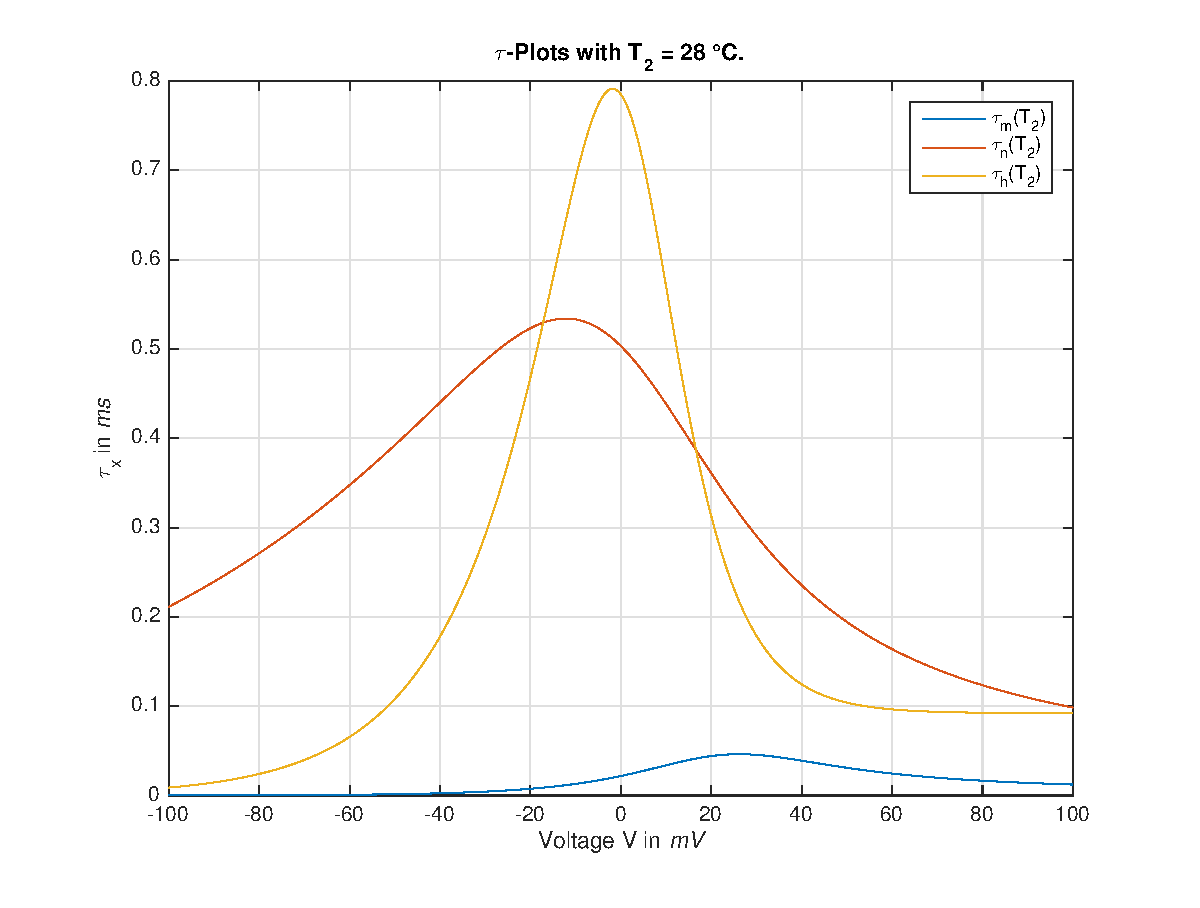
\includegraphics[width=0.45\linewidth]{Plots/tau_t_2}
\caption{$\tau$-plots for temperatures $T=6.3$\textcelsius~(left), and $T=28$\textcelsius~(right). The y-scale of the plot on the right hand side is smaller by a factor of ca. 10.}
\label{fig:tau_t_1}
\end{figure}

	\textbf{Interpretation: }The steady-state probabilities for open ion channels are denoted $m_{\infty}$, $n_{\infty}$ and $h_{\infty}$. As the membrane potential $V_m$ is shifted, such that $V = V_m - V_{rest}$, a positive value for $V$ indicates a depolarization of the membrane (see figure~\ref{fig:x_inf_plots}). Consequently, a negative value indicates a hyperpolarization. At the resting membrane potential $V = 0$ mV, almost none of the sodium-ion channels are open ($m_{\infty}<0.1$). At the same time, about 60 \% of the sodium-ion channels are not inactivated ($h_{\infty} \approx 0.6$). In contrast to that, around 30 \% of the potassium-ion channels are open ($n_{\infty} \approx 0.3$), meaning that the sodium conductance at rest is much smaller than the potassium conductance. By depolarizing the membrane (shifting $V$ positively), larger percentages of the Na+ and K+ channels are rapidly activated, while at the same time the number of inactivated Na+ gates increases ($h_{\infty}$ drops). A depolarization by around 70 mV results in an inactivation of virtually all Na+ channels (over 95 \%).\\
	At that point, the rates for the time constants $\tau$ become more important factors (see figure~\ref{fig:tau_t_1}): At resting membrane potential, $\tau_m$ is much smaller than the other two time constants (0.2 ms vs. 5.5 ms for $\tau_n$ and 8.5 ms for $\tau_h$. As a result, the sodium activation gates open much faster in response to depolarization compared to the other two gates, e.g. when stimulated by current injection. The opened sodium channels increase the inward flow of sodium ions, which in turn further depolarizes the cell membrane. If the initial stimulus was sufficiently high (resulting in a few mV of depolarization), the process becomes self-amplifying and results in the firing of an action potential.\\
	The potassium-ion channel activation gate and the sodium channel inactivation gate are slower by some milliseconds and thus lag behind. The potassium channels eventually (after the time lag) open and the sodium channels close by large numbers, repolarizing the membrane and bringing the membrane potential back to rest.\\\\
	
	
	\textbf{Note: }The rates for the time constants are significantly smaller for higher temperatures due to the \textit{RGT-Regel} (engl. Q10 temperature coefficient), which is a rule of thumb in chemical kinetics. The rule suggests that a rise in temperature by $10$ K results in an approximately two to four-times higher speed of the respective chemical reaction (figure~\ref{fig:tau_t_1}). \\
	
	
	\subsection{Hodgkin \& Huxley Neuron Model}
	\subsubsection{Experiments:}
	Hereby, \emph{Exp. 1} denotes the case described in 2.1.1 of the problem sheet. \emph{Exp. 2} denotes the case described in 2.1.2 of the problem sheet. 
For the plots of the membrane potential over time (1.), the gating constants m, n, h over time (2.), the current densities $i_{Na}$, $i_K$ over time (3.), the current densities $i_{Na}$, $i_K$ and $i_L$ over the membrane potential (4.), \emph{see figures~\ref{fig:hodgkin_huy_Vm}, \ref{fig:exp1_mnh}, \ref{fig:exp1_currents_time}, \ref{fig:exp1_phaseplot} respectively.}
\begin{figure}[h]
\centering
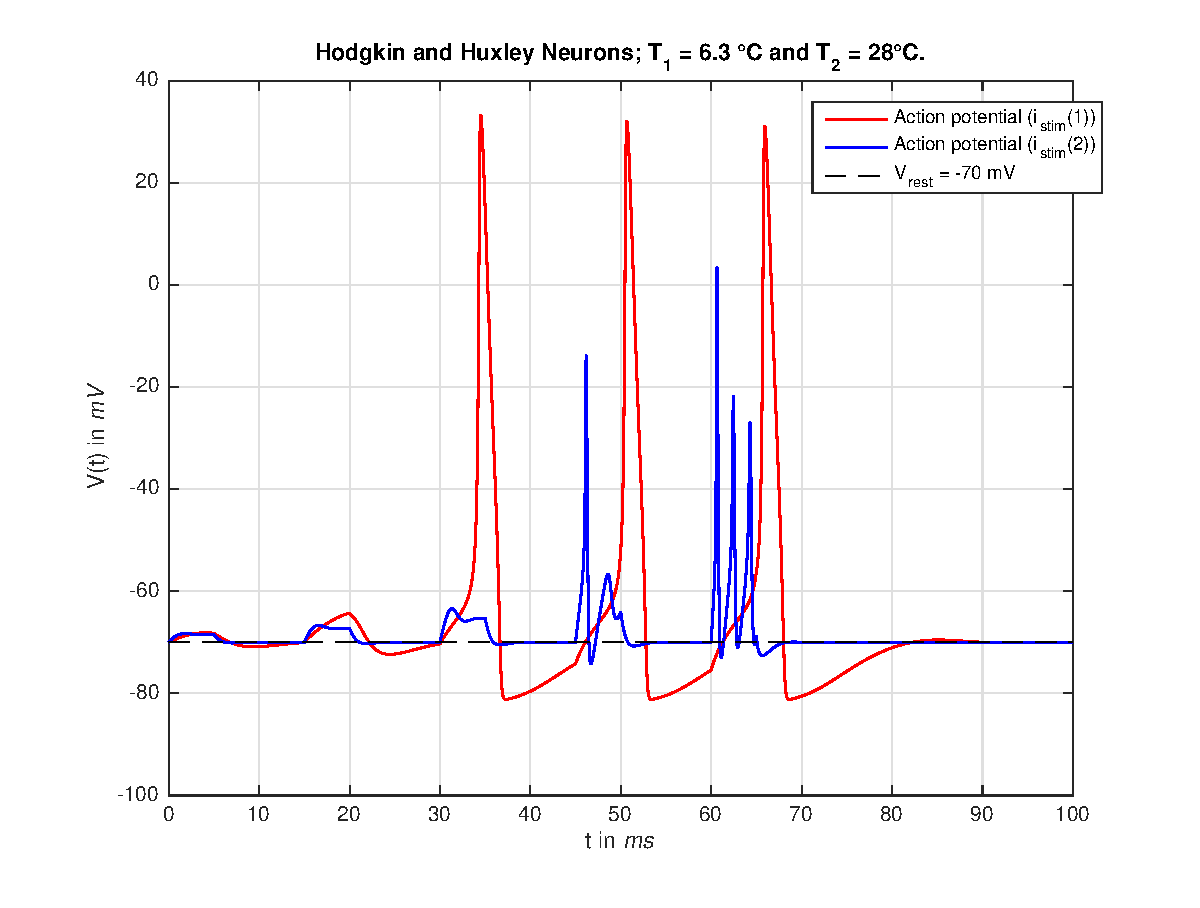
\includegraphics[width=0.7\linewidth]{Plots/hodgkin_huy_Vm}
\caption{Membrane potential $V_m$ for different input stimuli at different temperatures.}
\label{fig:hodgkin_huy_Vm}
\end{figure}
\begin{figure}[h]
\centering
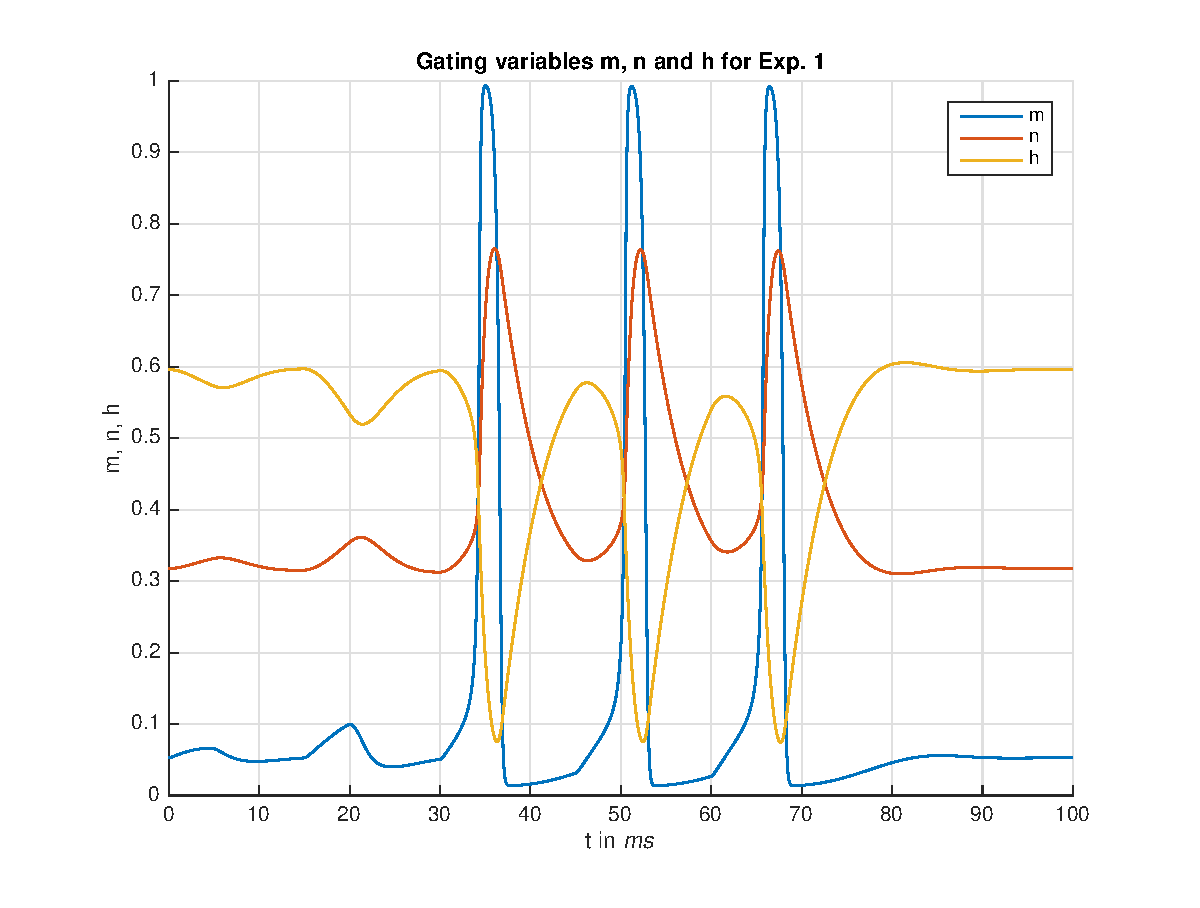
\includegraphics[width=0.45\linewidth]{Plots/exp1_mnh}
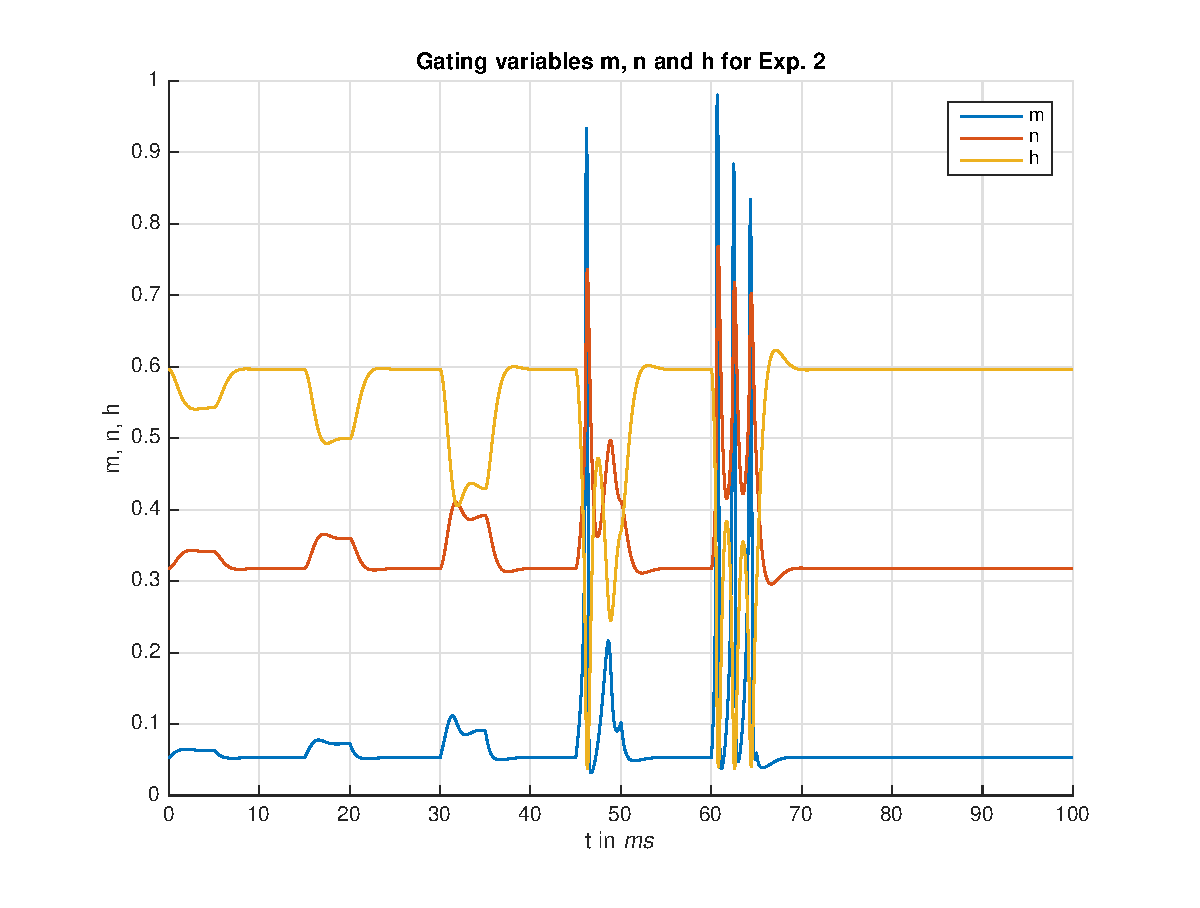
\includegraphics[width=0.45\linewidth]{Plots/exp2_mnh}
\caption{Gating constants m, n, h for Exp. 1 (left) and Exp. 2 (right).}
\label{fig:exp1_mnh}
\end{figure}

\begin{figure}[h]
\centering
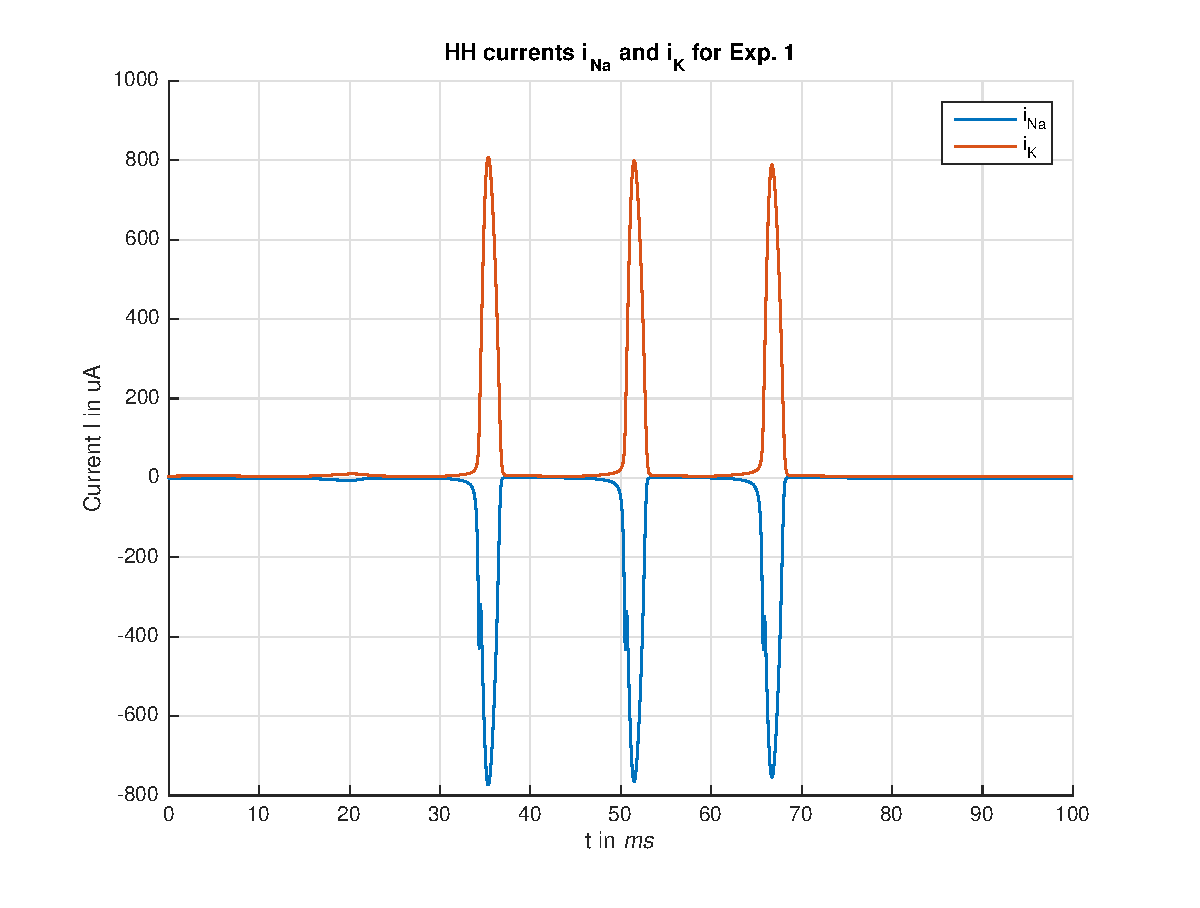
\includegraphics[width=0.45\linewidth]{Plots/exp1_currents_time}
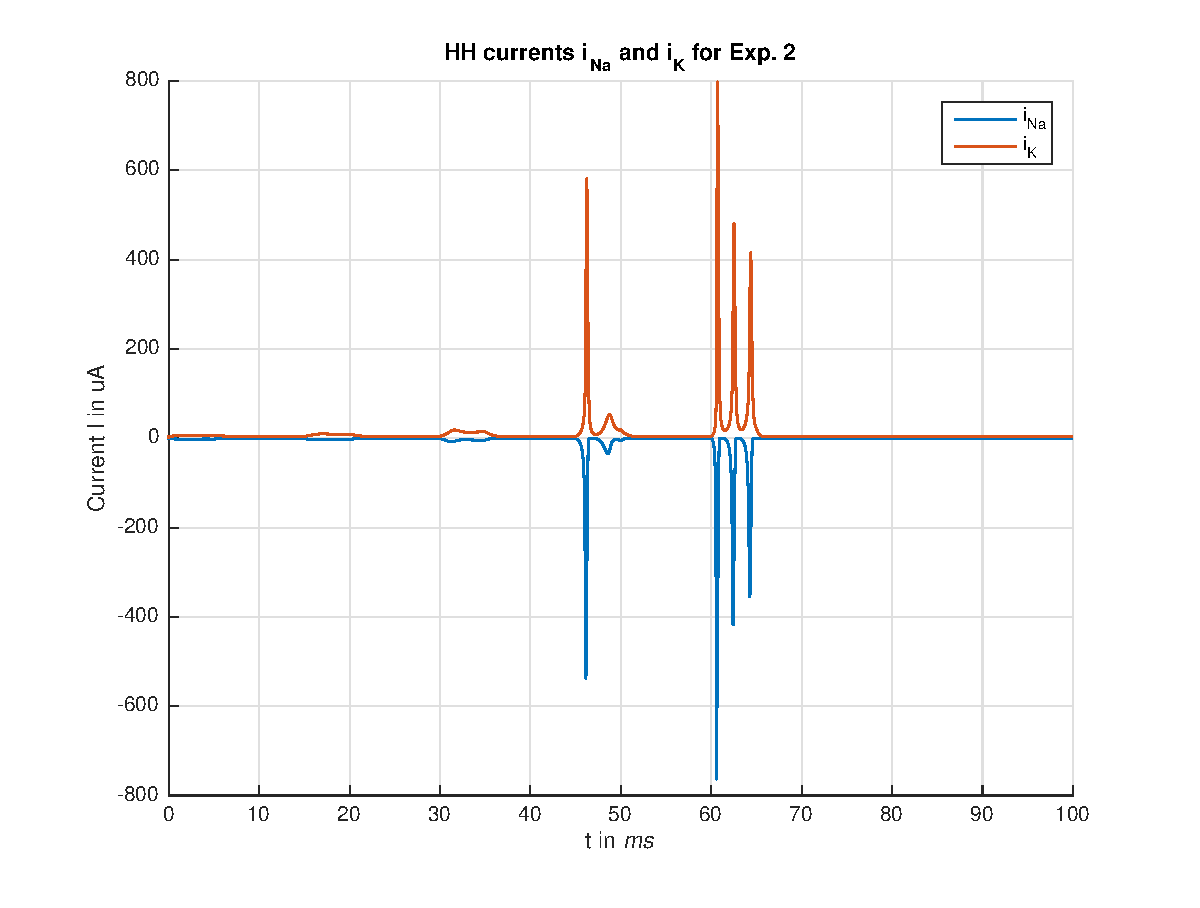
\includegraphics[width=0.45\linewidth]{Plots/exp2_currents_time}
\caption{Current densities $i_{Na}$ and $i_K$ over time for Exp. 1 (left) and Exp. 2 (right).}
\label{fig:exp1_currents_time}
\end{figure}

\begin{figure}[h]
\centering
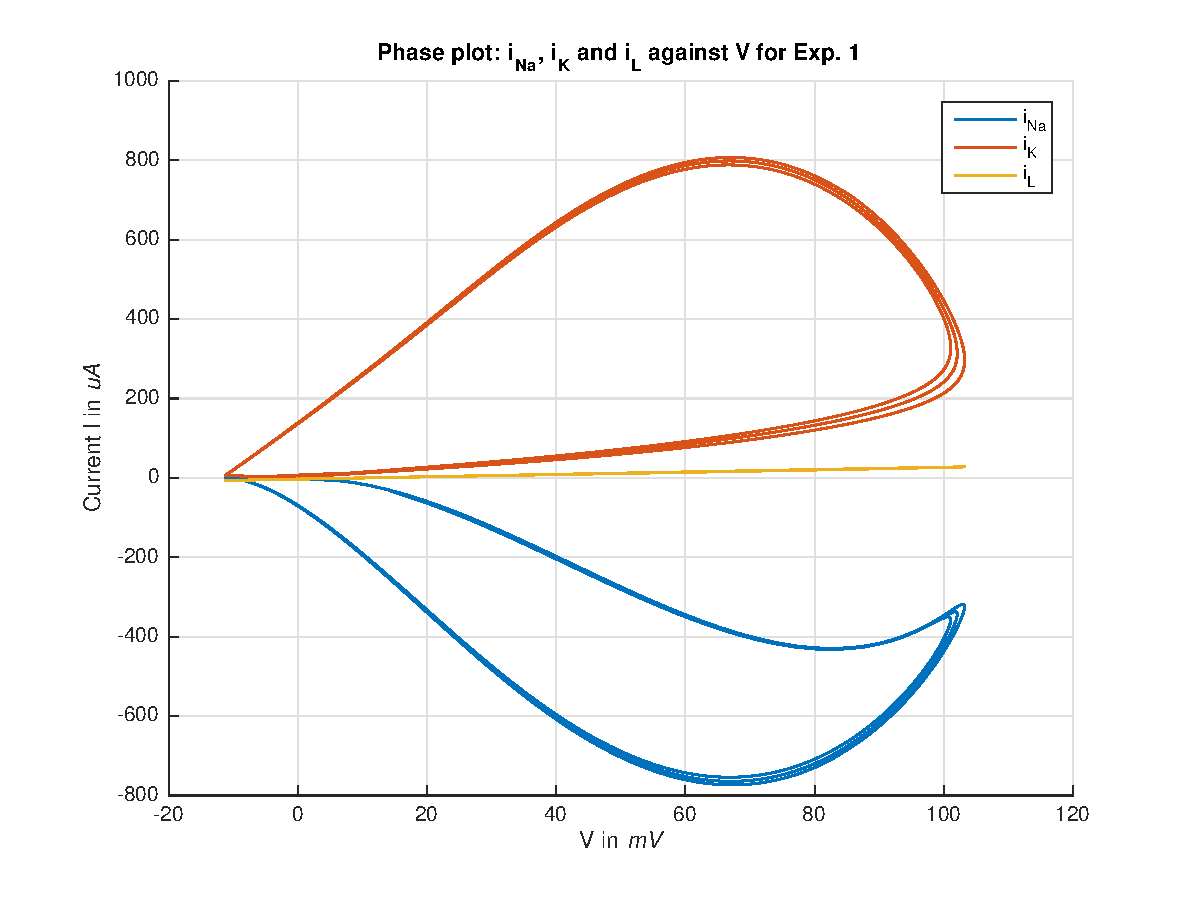
\includegraphics[width=0.45\linewidth]{Plots/exp1_phaseplot}
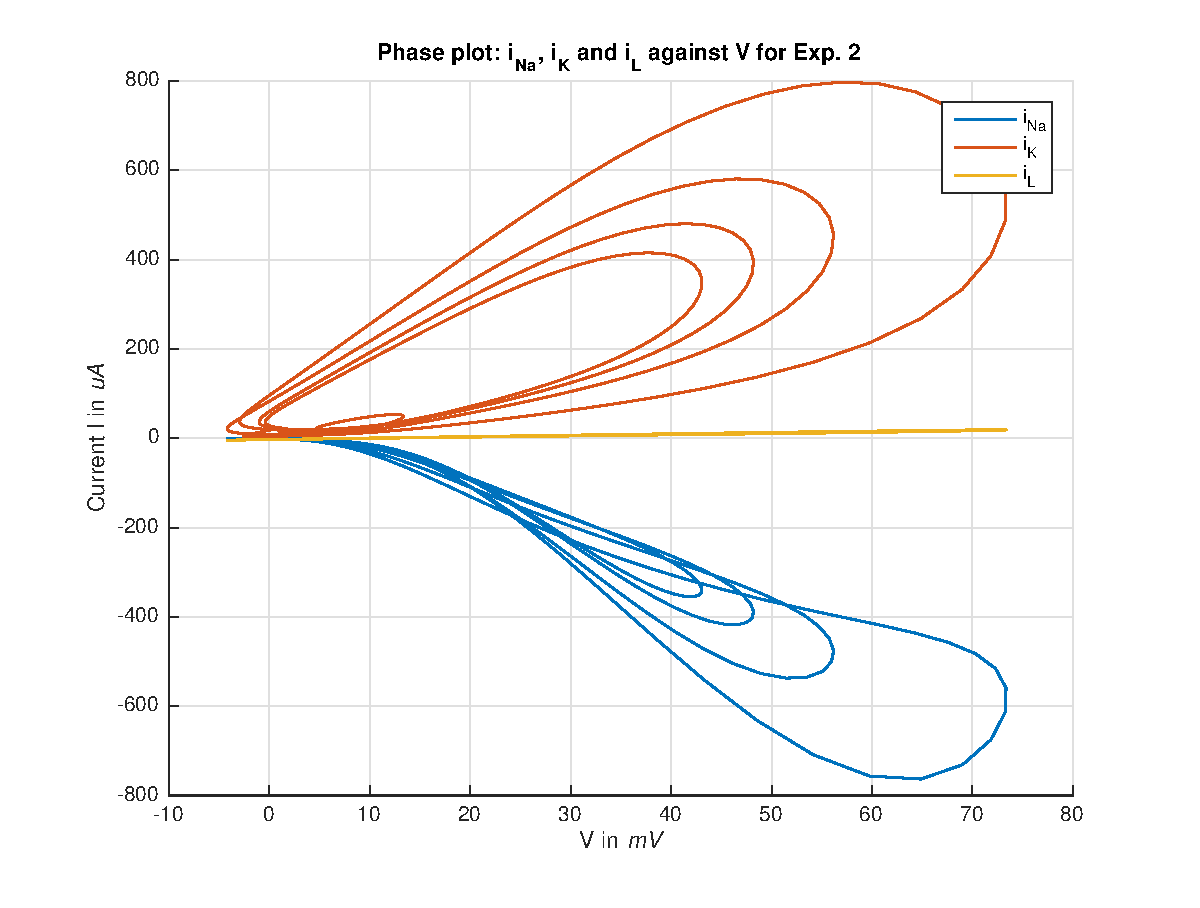
\includegraphics[width=0.45\linewidth]{Plots/exp2_phaseplot}
\caption{Plots of the current densities $i_{Na}$, $i_K$ and $i_L$ against the membrane potential $V$ for Exp. 1 (left) and Exp. 2 (right) (phase plots).}
\label{fig:exp1_phaseplot}
\end{figure}
\subsubsection{Analysis of the results}
\begin{itemize}
	\item \textit{Describe the differences between the results at 6.3 \textcelsius~ and 28 \textcelsius}.\\
	Hodgkin and Huxley performed their voltage clamp experiments at 6.3\textcelsius. Higher temperatures affect the reversal potentials since the Nernst equation is temperature dependent, but by far more dramatic is its influence on the rate constants: higher temperatures lead to significantly lower time constants (compare figures in figure~\ref{fig:tau_t_1}), decreased amplitudes and higher firing rates (figure~\ref{fig:hodgkin_huy_Vm}). 
	
	\item \textit{How is an action potential generated and what is the role of the different currents
and gating variables?}\\
	See explanation in previous problem (1) above; and additionally: The Na+-current is responsible for depolarization while the K+-current repolarizes the membrane, i.e. restores the resting membrane potential by the inward flow of K+ ions. For the role of the gating variables, see problem 1. 
	
	\item \textit{Explain why consecutive action potentials decrease in amplitude (at 28\textcelsius).}\\
	That question has also already been partly answered in problem 1. Furthermore, the inward Na+ ion flow is critical for depolarization and thus for the generation of an action potential. With an increased firing rate (higher temperature), the recovery of the Na+ ion concentration does not keep track with the firing rate. As the concentration of the sodium ions is reduced by subsequent action potentials, the action potentials become smaller. 
	
	
	\item \textit{How can you interpret the phase plot?}\\
	The potassium current $i_K$ is in the upper half plan of the plot (only positive current densities) and the sodium current $i_{Na}$ is only in the lower plot plane (only negative current densities), which is pretty obvious as Na+ ions flow into the cell, and K+ flow outside the cell when the respective channels are open. This hold for both plots in figure~\ref{fig:exp1_phaseplot}. The respective closed ellipses are better visible in the plot for the higher temperature on the right hand side. Time dependencies are not visible in the phase plots, as the current densities are plotted against the membrane potential. However, it is noticeable that each action potential follows an ellipse in the plot respectively: after having risen initially, the current goes back without 'jumps' to the initial state. We could now further investigate the leak current $i_L$, as it is very small in the plots. At this point, we can only say that the leak current is in the upper plane and rises unsubstantially with the membrane potential. 
	
	
	
	\item \textit{Explain the differences between the LIF and the HH model, why would you implement one or the other?}\\
	The HH model of the neuron is based on real physiological dynamic features of real biological neurons. However, it is highly non-linear, exhibits a large number of variables and is therefore hard to analyze mathematically and computationally complex.\\
	The LIF neuron model is a rather simple model that is not able to reproduce various features of real biological neurons. However, it is mathematically simple and an implementation of even larger networks of LIF neurons is computationally feasible. In contrast to that, HH models are less convenient for simulations of bigger networks but more for the study of biological properties. 
	
\end{itemize}



	
	
	

\end{document}